\documentclass[tikz,border=8pt]{standalone}
\begin{document}
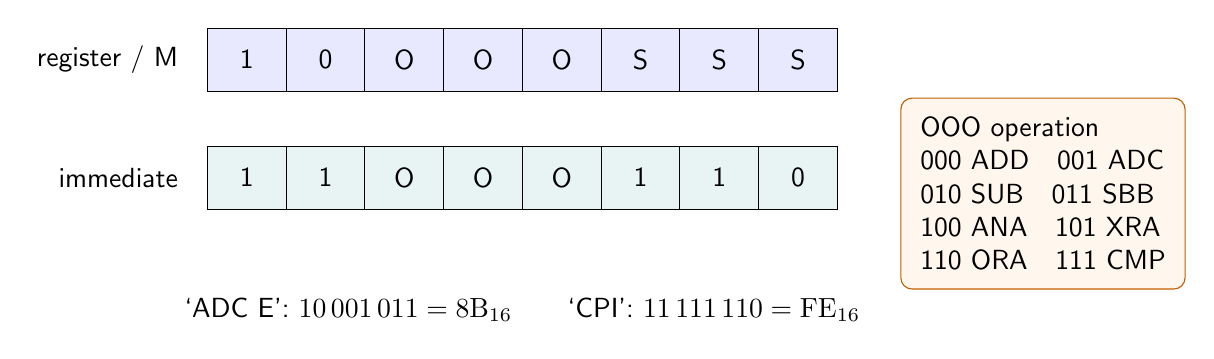
\begin{tikzpicture}[font=\sffamily,x=1cm,y=1cm]
\node[anchor=east] at (-.25,3.7){register / M};
\foreach \x/\v in {0/1,1/0,2/O,3/O,4/O,5/S,6/S,7/S}{\draw[fill=blue!9] (\x,3.3) rectangle ++(1,.8);\node at (\x+.5,3.7){\v};}
\node[anchor=east] at (-.25,2.2){immediate};
\foreach \x/\v in {0/1,1/1,2/O,3/O,4/O,5/1,6/1,7/0}{\draw[fill=teal!9] (\x,1.8) rectangle ++(1,.8);\node at (\x+.5,2.2){\v};}
\node[anchor=west,draw=orange!75!black,rounded corners,fill=orange!7,align=left,inner sep=7pt] at (8.8,2.0) {OOO operation\\000 ADD\quad001 ADC\\010 SUB\quad011 SBB\\100 ANA\quad101 XRA\\110 ORA\quad111 CMP};
\node[below,align=center] at (4,.8) {`ADC E': $10\,001\,011=8\mathrm{B}_{16}$\qquad `CPI': $11\,111\,110=\mathrm{FE}_{16}$};
\end{tikzpicture}
\end{document}
